\documentclass[11pt]{article}
\usepackage[margin=1in]{geometry}
\usepackage{amsmath,amssymb}
\usepackage{graphicx}
\usepackage{booktabs}
\usepackage{microtype}
\usepackage[round]{natbib}
\usepackage[hidelinks]{hyperref}
\usepackage{xcolor}
\usepackage{caption}
\captionsetup{font=small,labelfont=bf}

\newcommand{\divg}{\mathrm{div}}

\title{\textbf{Noise or Sensitivity? Disentangling Prompt Perturbation Effects
from Intrinsic Nondeterminism in Chained LLM Agents}}
\author{Venkata Koushik\\
\texttt{venkatakoushik777@gmail.com}}
\date{July 18, 2026}

\begin{document}
\maketitle

\begin{abstract}
Prompt sensitivity (the tendency of large language models to produce
different outputs under semantically equivalent prompt rewordings) is well
documented for single models, but its behavior in multi-agent pipelines,
where one agent's output becomes the next agent's input, has not been
measured. We ask whether paraphrase-induced divergence compounds with chain
depth, and introduce the control condition that turns out to be decisive:
repeated runs of \emph{unperturbed} chains at temperature~0, which isolate
intrinsic sampling nondeterminism from prompt-attributable variance. Across
1{,}470 runs of three 4-stage pipelines (summarization, research planning,
code review) with 118 validated paraphrases (120 generated; 2 degenerate
duplicates of their base prompt detected and excluded, with the 15 affected
runs), we find that (1)~apparent divergence growth with depth is largely
\emph{not} a prompt effect: unperturbed chains amplify intrinsic
nondeterminism with depth, reaching a 40\% catastrophic-divergence rate at
depth~3 on the most open-ended task with no perturbation at all, a rate not
distinguishable from perturbed runs given our control sample size
($p=0.31$, $n_{\mathrm{control}}=5$), implying that intrinsic nondeterminism
accounts for at minimum the majority of the observed catastrophe rate;
(2)~the residual paraphrase-attributable effect is modest and does not
compound: excess divergence over the noise floor stays flat or declines
with depth; (3)~perturbation \emph{position} matters more than count of
downstream stages: perturbing the first agent yields significantly more
final-output divergence than perturbing the last ($0.155$ vs $0.116$,
Mann--Whitney $p = 2.1\times10^{-10}$, Cliff's $\delta = 0.246$); and
(4)~format-constrained final stages act as attractors that repair both noise
sources: our summarization pipeline's divergence \emph{decreases} with
depth (Spearman $\rho = -0.196$) and structured-output schema violations are
0\%. Our results caution that studies of prompt robustness in agent
pipelines must control for nondeterminism amplification, and suggest that
practitioners should invest prompt-hardening effort in early-position agents
and convergent final stages. Harness, prompts, raw runs, and analysis are
released for reproduction.\footnote{\url{https://github.com/koushik717/prompt-sensitivity-chains}}
\end{abstract}

\section{Introduction}

A growing share of LLM deployments are not single calls but \emph{chains}:
an extractor feeding a summarizer feeding an editor; an analyzer feeding a
reviewer feeding a report writer. Each stage consumes the previous stage's
output as input, so any instability in an early stage has, in principle, the
entire remaining pipeline through which to propagate. At the same time, a
well-replicated line of work shows that individual LLMs are surprisingly
sensitive to semantically irrelevant prompt variation: formatting,
phrasing, and paraphrase changes can swing single-model benchmark
performance by double digits
\citep{sclar2024,zhu2023,mizrahi2024,sun2023,cao2024}. The natural worry,
voiced but to our knowledge never measured, is multiplicative: if one agent
is prompt-sensitive, is a chain of four agents four times as fragile, or
worse?

This paper measures that question directly, and the measurement produces a
twist. The naive experiment (paraphrase one agent's system prompt, run the
chain, measure embedding divergence of the final output from a
canonical-prompt run) shows divergence growing with depth on two of our
three tasks, with catastrophic divergence (cosine divergence $>0.3$) spiking
from 0\% at depth~1 to 20\% at depth~3 in the pooled data. Reported alone,
that would read as confirmation of compounding prompt sensitivity.

It would be wrong. Our design includes a control arm that most prior
robustness studies omit: the \emph{same} chains, with \emph{canonical}
prompts at every position, run repeatedly at temperature~0. These
unperturbed repeats are not identical: temperature-0 decoding is not
deterministic in practice, with accuracy variation of up to 15\% documented
across nominally deterministic runs \citep{atil2024,ouyang2023,he2025}, and
the small token-level differences they contain are amplified by exactly the
same chain dynamics as paraphrase perturbations. On our most open-ended task
(research planning), unperturbed depth-3 chains reach a mean divergence of
0.297 and a 40\% catastrophic-divergence rate; the corresponding perturbed
runs reach 0.322 and 57\%, not distinguishable from the controls given our
control sample size (one-sided Mann--Whitney $p = 0.31$,
$n_{\mathrm{control}} = 5$). The depth-3 ``catastrophe spike'' is real, but
at minimum the majority of it is not a prompt-sensitivity effect: it is the
chain amplifying its own sampling noise. This extends the finding that
subtle nondeterminism compounds across turns in multi-turn conversation
\citep{laban2025} to the multi-agent setting, and it means that any study
attributing chained-output divergence to a manipulated variable must first
subtract the divergence the pipeline generates on its own.

With the noise floor subtracted, three clean findings remain.

\paragraph{Paraphrase sensitivity does not compound with depth.} Excess
divergence (perturbed mean minus control mean, within task~$\times$~depth
cells) is modest everywhere and roughly flat or declining: $+0.079 \to
+0.032$ across depths $1\to4$ for summarization, a steady ${\approx}+0.025$
for code review, and within noise for research planning. The pooled raw
trend (Spearman $\rho = 0.089$) is significant but tiny, and per-task trends
disagree in sign (code review $+0.34$, summarization $-0.20$), the opposite
of a universal amplification law.

\paragraph{Position beats depth.} Where the paraphrase lands matters more
than how many stages follow it in aggregate: perturbing the first agent
produces significantly more final divergence than perturbing the last
($0.155$ vs $0.116$; Mann--Whitney $p = 2.1\times10^{-10}$; Cliff's
$\delta = 0.246$). Because both position groups face identical intrinsic
noise, this comparison is naturally noise-robust.

\paragraph{Convergent stages repair.} Stages whose task is to check, edit,
or format into a fixed schema act as attractors: summarization divergence
\emph{decreases} with depth as the fact-checker and editor renormalize
drafts; the code-review pipeline's JSON-constrained report writer produced
zero schema violations across all perturbed depth-4 runs; and the depth-3
catastrophe rate collapses from 20\% to 2\% at depth~4 once the constrained
final stages run. This corroborates, from an orthogonal experimental angle,
the observation that deeper cascades can \emph{reduce} factual error scores
\citep{hallucascade2026}.

\paragraph{Contributions.}
\begin{enumerate}
  \item \textbf{To our knowledge, the first controlled separation of
  paraphrase-induced divergence from intrinsic sampling nondeterminism in
  chained LLM pipelines}, showing that what appears to be compounding prompt
  sensitivity is largely nondeterminism amplification: unperturbed
  temperature-0 chains reach catastrophic divergence rates of 40\% at
  depth~3 on open-ended tasks.
  \item \textbf{A perturbation-position effect}: early-agent paraphrases
  cause significantly more final-output divergence than late-agent
  paraphrases ($p = 2.1\times10^{-10}$, Cliff's $\delta = 0.246$), with
  practical implications for where prompt-hardening effort pays off.
  \item \textbf{Evidence of convergent-stage repair}: constrained final
  stages attenuate both noise sources, independently corroborating
  cascade-reduction findings from hallucination tracking.
\end{enumerate}

We release the full harness (checkpointed runner, validated paraphrase sets,
versioned judge rubrics, analysis pipeline), all 1{,}470 raw run
transcripts, and the processed data.

\section{Related Work}

\paragraph{Single-model prompt sensitivity.} That LLMs are sensitive to
semantically irrelevant prompt variation is by now well established.
PromptBench \citep{zhu2023} measures robustness to adversarial prompt
perturbations at character, word, sentence, and semantic levels across 8
tasks; \citet{sclar2024} show that spurious formatting features
alone (separators, capitalization, spacing) induce large performance
swings; \citet{sun2023} find that instruction-tuned models degrade on unseen
paraphrases of their task instructions; and \citet{cao2024} document gaps of
up to 45 points between best- and worst-performing paraphrases of the same
query, arguing for worst-prompt evaluation as a lower bound.
\citet{mizrahi2024} make the methodological case that single-prompt
evaluation is unreliable, from 6.5M evaluation instances. All of this work
evaluates a \emph{single} model per call. Whether sensitivity compounds,
attenuates, or transforms when a prompt-sensitive model's output becomes
another prompt-sensitive model's input is the question this line of work
leaves open, and the one we address.

\paragraph{Error propagation in multi-agent LLM systems.} A rapidly growing
2026 literature studies how errors move through agent pipelines. Closest to
us, the Hallucination Cascade study \citep{hallucascade2026} tracks
claim-level factual inconsistency across sequential agents and finds that
deeper cascades \emph{reduce} normalized hallucination scores
($0.422 \to 0.272$ over three agents) at a small cost in factual
preservation, independently corroborating, via a different measurement
(claim-level factuality vs.\ output-embedding divergence), the
convergent-stage repair we observe. From Spark to Fire \citep{spark2026}
models collaboration as a dependency graph and shows that a single injected
atomic error seed can propagate to system-level false consensus, identifying
cascade amplification and topological sensitivity as vulnerability classes.
MAS-FIRE \citep{masfire2026} injects 15 fault types into MAS pipelines for
reliability evaluation, and AgentAsk \citep{agentask2025} attributes MAS
underperformance to errors at inter-agent message handoffs, proposing
edge-level clarification. The key difference in our design: these works
perturb with \emph{errors}: injected faults, tracked hallucinations,
corrupted messages. Our perturbation is \emph{benign by construction}
(validated semantically equivalent paraphrases), so any divergence we
measure is attributable to sensitivity rather than to the propagation of a
defect. And none of these works measures its pipeline's unperturbed variance
floor, which our results show can dominate the measured effect.

\paragraph{Nondeterminism of ``deterministic'' LLM inference.}
\citet{atil2024} systematically document accuracy variation of up to 15\%
(and best-to-worst output gaps up to 70\%) across runs of LLMs configured to
be deterministic; \citet{ouyang2023} report the same phenomenon for ChatGPT
code generation. The mechanism is now well understood: serving-time
batch-size variation interacts with non-batch-invariant kernels
\citep{he2025}. Most relevantly, \citet{laban2025} show that in multi-turn
conversation, temperature-0 decoding still yields high unreliability because
subtle nondeterminism compounds across tokens and turns. Our control
condition extends this compounding result from the multi-turn single-agent
setting to multi-agent chains, and quantifies it per task and depth,
showing it grows to catastrophic levels (40\% of unperturbed depth-3 runs on
our most open-ended task) exactly where a naive reading would attribute the
failures to prompt sensitivity.

\paragraph{Positioning.} The sensitivity literature perturbs prompts but
tests single models; the cascade literature tests chains but perturbs with
errors; the nondeterminism literature perturbs nothing but stops at single
calls or single-agent conversations. To our knowledge no prior work runs
benign prompt perturbations through multi-stage pipelines \emph{against a
matched unperturbed control}, which is precisely the design needed to
separate the two variance sources. In our data, that separation reverses
the naive conclusion.

\section{Method}

\subsection{Pipelines and tasks}

Three 4-role pipelines, truncatable at depth $k \in \{1,2,3,4\}$ (agent
$k$'s output is the final output):

\begin{table}[h]
\centering\small
\begin{tabular}{lll}
\toprule
Task & Chain & Final output \\
\midrule
summarization & extractor $\to$ summarizer $\to$ fact\_checker $\to$ editor & ${\sim}100$-word summary \\
research\_plan & scoper $\to$ planner $\to$ critic $\to$ finalizer & structured plan document \\
code\_review & analyzer $\to$ reviewer $\to$ security\_checker $\to$ report\_writer & JSON report \\
\bottomrule
\end{tabular}
\caption{Task pipelines. The code-review report must be a JSON object with
keys \texttt{summary}, \texttt{issues}, \texttt{severity}.}
\end{table}

Five fixed inputs per task, held constant across all conditions.

\subsection{Perturbations}

Ten paraphrases per base system prompt (120 total) were generated by
\texttt{claude-sonnet-4-6} at temperature 0.9 and validated by embedding
similarity (all-MiniLM-L6-v2 cosine $\geq 0.85$ vs.\ base). Six paraphrases
below threshold were manually reviewed and accepted (stylistic reframing,
meaning preserved; review documented in the repository). A post-hoc identity
check found 2 of the 120 generated ``paraphrases'' to be byte-identical
(after whitespace/case normalization) to their base prompts; these were
excluded, and the 15 runs perturbed with them were dropped from the
perturbed condition (they are unperturbed chains), leaving 118 valid
paraphrases and 1{,}335 analyzed perturbed runs. Exactly \textbf{one}
agent's prompt is perturbed per run, at position first, middle
($\lfloor \mathrm{depth}/2 \rfloor$), or last (deduplicated per depth).

\subsection{Conditions}

\begin{itemize}
  \item \textbf{baseline}: canonical prompts at every position; the
  reference run per (task, input, depth).
  \item \textbf{perturbed}: one position paraphrased: 3 tasks $\times$ 5
  inputs $\times$ 10 paraphrases $\times$ $\sum$ positions(depth) $=$
  1{,}350 runs (15 excluded as pseudo-perturbed per \S3.2; \textbf{1{,}335
  analyzed}).
  \item \textbf{control}: canonical prompts, 5 repeats at temperature 0
  per (task, depth) on one fixed input $=$ 60 runs; quantifies intrinsic
  nondeterminism (the noise floor).
\end{itemize}

Total: 1{,}470 runs / 4{,}200 agent calls; zero failed runs after retries;
agents \texttt{claude-haiku-4-5-20251001} at temperature 0, max 1{,}024
tokens; total agent-call cost \$13.68 (from logged per-call token counts).

\subsection{Metrics}

\begin{itemize}
  \item \textbf{Divergence}: $1 - $ cosine similarity (all-MiniLM-L6-v2)
  between the final outputs of a perturbed (or control) run and its
  same-(task, input, depth) baseline run.
  \item \textbf{Catastrophic divergence}: divergence $> 0.3$ (transcript
  inspection confirms this threshold separates rewordings from semantic
  derailment; see \S5).
  \item \textbf{Excess divergence}: perturbed cell mean $-$ control cell
  mean within (task, depth), the paraphrase-attributable component.
  \item \textbf{Task success}: LLM-as-judge (\texttt{claude-sonnet-4-6},
  temperature 0), depth-appropriate versioned rubrics (v2) grading the
  artifact the depth-$k$ chain actually produces; judge model $\neq$ agent
  model; 10\% double-judged $\to$ 96.3\% exact agreement, mean $|\Delta|$
  0.04 ($n = 164$).
  \item \textbf{Schema violations}: JSON parse $+$ required-key check
  (code\_review, depth 4 only).
\end{itemize}

Statistics: bootstrap 95\% CIs (5{,}000 resamples); Spearman trend tests on
divergence and on the catastrophe indicator; Mann--Whitney $U$ $+$ Cliff's
$\delta$ for the position contrast. Effect sizes are reported alongside
$p$-values throughout.

\section{Results}

\begin{figure}[t]
\centering
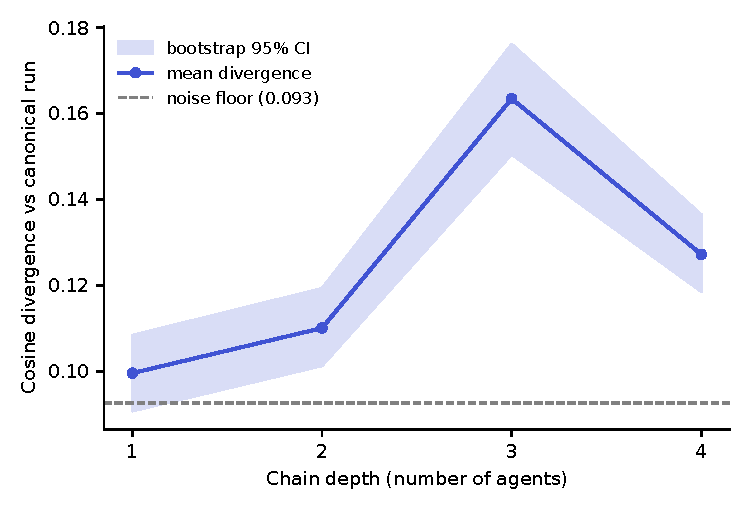
\includegraphics[width=0.78\textwidth]{divergence_vs_depth.pdf}
\caption{Mean embedding divergence of perturbed runs vs.\ chain depth,
pooled across tasks, with bootstrap 95\% CIs.}
\label{fig:divdepth}
\end{figure}

\begin{figure}[t]
\centering
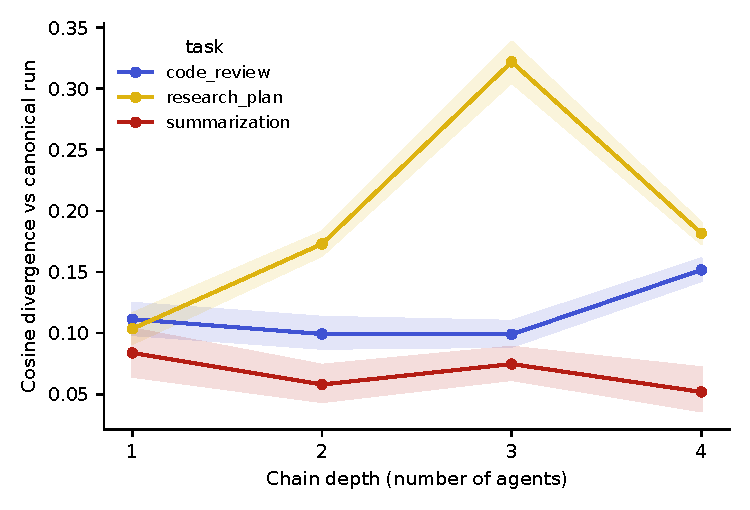
\includegraphics[width=0.78\textwidth]{per_task_curves.pdf}
\caption{Per-task divergence vs.\ depth. The sign of the depth trend
differs by task: rising for code review and research planning, falling for
summarization.}
\label{fig:pertask}
\end{figure}

\subsection{Raw divergence grows weakly and non-uniformly with depth}

Pooled across tasks, mean divergence rises from 0.0996 [95\% CI 0.0908,
0.1084] at depth 1 to 0.1272 [0.1186, 0.1364] at depth 4, a $1.28\times$
amplification, with a Spearman trend of $\rho = 0.089$
($p = 1.2\times10^{-3}$): statistically detectable, but far from the
multiplicative compounding the fragility hypothesis predicts
(Fig.~\ref{fig:divdepth}). The pooled number moreover conceals qualitative
disagreement between tasks (Fig.~\ref{fig:pertask}): divergence
\emph{rises} with depth for code review ($\rho = 0.339$,
$p = 1.5\times10^{-13}$) and research planning ($\rho = 0.225$,
$p = 2.2\times10^{-6}$) but \emph{falls} for summarization
($\rho = -0.196$, $p = 2.8\times10^{-5}$), whose fact-checking and editing
stages progressively pull perturbed drafts back toward the baseline. There
is no universal amplification law to report; the sign of the depth effect is
a property of the pipeline's stage structure, not of chaining itself.

\subsection{The catastrophe spike is largely nondeterminism, not
sensitivity}

Pooled catastrophe rate: 0\% (d1) $\to$ 2.3\% (d2) $\to$ 20.0\% (d3) $\to$
2.3\% (d4); the depth-3 spike is driven entirely by research\_plan (57.2\%).
Control chains at the same cell: mean divergence 0.297, catastrophe rate
40\%, vs.\ perturbed 0.322, not distinguishable given the control sample
size (one-sided Mann--Whitney $p = 0.31$, $n_{\mathrm{control}} = 5$). At
minimum, intrinsic nondeterminism accounts for the majority of the observed
catastrophe rate at this cell; our control arm is too small to bound any
residual paraphrase contribution tightly.

Notably, the noise floor is strongly \emph{task-dependent}: control
divergence is near zero for summarization at every depth (0.005--0.032),
moderate for code review (0.072--0.126), and large and depth-growing for
research planning ($0.066 \to 0.297$ across d1$\to$d3). The same chain
architecture, run on the same infrastructure at the same temperature,
produces intrinsic output variance spanning nearly two orders of magnitude
depending on how open-ended the stage artifacts are. This is itself a
methodological result: single-number robustness claims about ``LLM chains''
are underdetermined without specifying the task's constraint structure,
because the denominator against which any perturbation effect must be
judged varies by task and depth.

\subsection{Excess (paraphrase-attributable) divergence does not compound}

Subtracting each (task, depth) cell's control mean from its perturbed mean
isolates the component of divergence attributable to the paraphrase. This
excess is modest everywhere and shows no depth amplification in any task:
for summarization it \emph{declines} from $+0.079$ (d1) to $+0.032$ (d4);
for code review it holds nearly constant at ${\approx}+0.025$ across all
four depths; for research planning it fluctuates within the noise ($+0.038$
at d1 to $-0.037$ at d4, a negative excess, i.e.\ perturbed runs diverging
\emph{less} than unperturbed controls at depth 4). With $n = 5$ controls per
cell these excesses are descriptive rather than tightly estimated, but their
pattern is uniform: whatever divergence paraphrases inject, the chain does
not multiply it.

\subsection{Position, not depth, is where prompt wording matters}

Restricting to depths $\geq 2$ where both positions exist, perturbing the
\emph{first} agent yields a mean final divergence of 0.1554 ($n = 450$)
against 0.1163 ($n = 440$) for the \emph{last} agent, a significant
difference (Mann--Whitney $U$, $p = 2.1\times10^{-10}$) with a
small-to-medium effect size (Cliff's $\delta = 0.246$). Restricting to depth
$\geq 3$ where all three positions exist, the ordering is monotone in
position: first $0.169 >$ middle $0.138 >$ last $0.129$. Because first- and
last-position groups within a cell face identical intrinsic noise, this
contrast is naturally robust to the noise-floor concerns of \S4.2. The
practical reading: a paraphrase that lands early has its perturbation
propagated, reinterpreted, and built upon by every subsequent stage, while a
late paraphrase can only re-style the nearly finished artifact.

\subsection{Convergent stages repair both noise sources}

\begin{figure}[t]
\centering
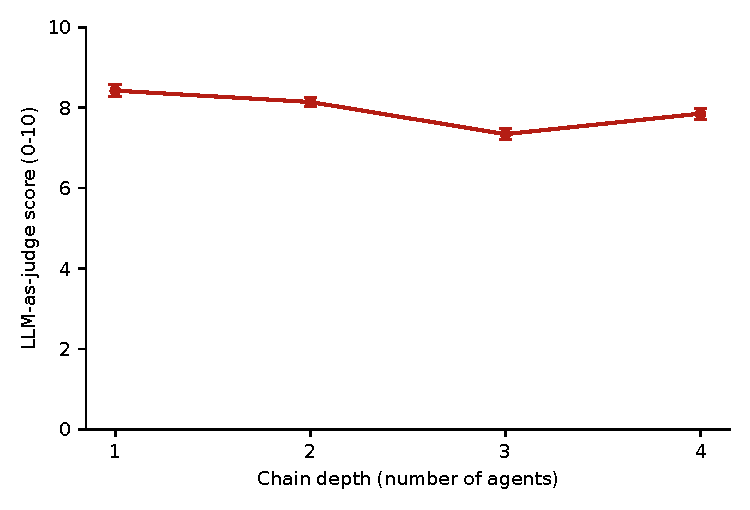
\includegraphics[width=0.78\textwidth]{success_vs_depth.pdf}
\caption{LLM-as-judge success scores (0--10, depth-appropriate rubrics)
vs.\ depth. The dip at depth 3 coincides with the open-ended critic stage;
scores recover at depth 4 when the constrained finalizer runs.}
\label{fig:success}
\end{figure}

\begin{figure}[t]
\centering
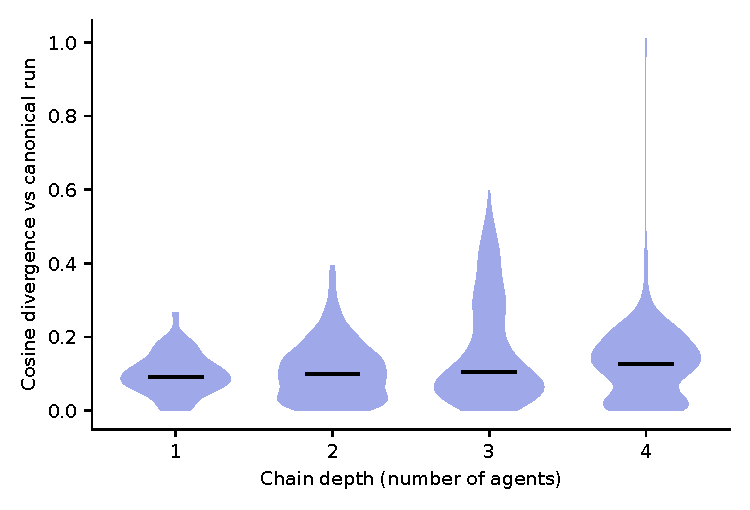
\includegraphics[width=0.78\textwidth]{divergence_violins.pdf}
\caption{Distribution of divergence by depth (violin plots). Depth
increases the tails far more than the bulk of the distribution.}
\label{fig:violins}
\end{figure}

Three independent observations triangulate the same mechanism. First, the
pooled catastrophe rate collapses from 20.0\% at depth 3 to 2.3\% at depth
4: adding the final, most format-constrained stage (editor / finalizer /
report writer) \emph{reduces} catastrophic divergence. Second,
summarization's negative depth trend (\S4.1) shows repair acting on
paraphrase perturbations specifically. Third, the structured-output check is
perfect: 0\% schema violations across all perturbed depth-4 code-review
runs: no paraphrase anywhere in the chain ever broke the final JSON
contract. Judge scores tell the same story from the quality side
(Fig.~\ref{fig:success}): mean score dips at depth 3 (7.34 [7.20, 7.48])
exactly where the open-ended critic stage maximizes divergence, then
recovers at depth 4 (7.85 [7.71, 7.99]). Constrained convergent stages act
as attractors in output space, a cheap architectural lever for chain
reliability, and one that corroborates the cascade-depth hallucination
reduction reported by \citet{hallucascade2026} from a different measurement
angle.

\section{Case study: a cascade failure}

Run \texttt{summarization|sum\_4|d4|p2|middle} (divergence 1.010, the grid
maximum): a paraphrase of the \emph{fact-checker} prompt led it to output an
analysis \emph{about} the draft rather than a corrected draft; the
downstream editor, receiving analysis instead of a summary, declined to edit
and asked for the missing summary, producing a final output unrelated to
the source article. The failure is qualitative and structural (a
role-contract violation between stages), not a gradual drift. Full
transcripts of the failed and baseline runs are included in the released
data.

\section{Limitations}

\begin{itemize}
  \item Single agent-model family (Claude Haiku 4.5) and one embedding model
  (MiniLM); effect sizes may differ across model families and embedders.
  \item Three tasks, five inputs each; task heterogeneity in our own results
  warns against over-generalizing any single trend.
  \item The control arm is small (5 repeats per task $\times$ depth cell; 60
  runs total), sufficient to reveal the noise floor's magnitude and depth
  trend, not to tightly bound it. The perturbed-vs-control comparison at the
  critical cell is correspondingly low-powered ($n_{\mathrm{control}} = 5$).
  \item The catastrophe threshold (0.3) is a single operating point chosen
  from transcript inspection; results are reproducible under nearby
  thresholds with the released analysis code.
  \item Paraphrases were LLM-generated and initially LLM-validated (a
  potential circularity for an LLM-sensitivity study, documented in the
  repository); a full human review of all 118 active paraphrases was
  subsequently performed by an author, confirming meaning preservation.
  \item LLM-as-judge scores, though reliable (96.3\% exact agreement), share
  training lineage with the agent model's vendor.
  \item Our chains are limited to 4 stages; whether the position effect and
  convergent-stage repair we observe persist, saturate, or reverse in much
  longer chains (tens to hundreds of agents) is an open question we did not
  test. Large-scale multi-agent systems have been studied at this scale for
  coordination quality and emergent behavior (e.g.\ a 25{,}000-run study of
  coordination protocols across 4--256 agents \citep{selforganizing2026} and
  MegaAgent's autonomous systems scaling to hundreds of agents
  \citep{megaagent2024}), but, to our knowledge, no prior work measures how a
  benign prompt perturbation propagates through chains at this scale. Whether
  the position effect strengthens, saturates, or is swamped by other noise
  sources as chain length grows by an order of magnitude or more is a natural
  and, we think, important direction for future work.
\end{itemize}

\section{Conclusion}

In four-stage LLM pipelines, semantically equivalent prompt rewordings do
not compound into runaway divergence: chains amplify their own sampling
nondeterminism far more than they amplify paraphrase perturbations, and
constrained late stages repair both. Robustness engineering for agent chains
should therefore (a)~control for intrinsic nondeterminism before attributing
divergence to any manipulated variable, (b)~invest prompt-hardening effort
in early-position agents, and (c)~treat constrained, convergent final stages
as a cheap reliability mechanism.

\section*{Acknowledgments}

The author thanks Thai Le for feedback on an earlier draft of this paper,
including the observation that the scaling question addressed in
Section~6's final limitation is where this line of work becomes most
interesting.

\begin{thebibliography}{13}

\bibitem[Zhu et al.(2023)]{zhu2023}
Zhu, K., et al. 2023.
\newblock PromptBench: Towards Evaluating the Robustness of Large Language
Models on Adversarial Prompts.
\newblock arXiv:2306.04528.

\bibitem[Sclar et al.(2024)]{sclar2024}
Sclar, M., Choi, Y., Tsvetkov, Y., Suhr, A. 2024.
\newblock Quantifying Language Models' Sensitivity to Spurious Features in
Prompt Design (or: How I learned to start worrying about prompt formatting).
\newblock ICLR 2024. arXiv:2310.11324.

\bibitem[Sun et al.(2023)]{sun2023}
Sun, J., et al. 2023.
\newblock Evaluating the Zero-shot Robustness of Instruction-tuned Language
Models.
\newblock arXiv:2306.11270.

\bibitem[Cao et al.(2024)]{cao2024}
Cao, B., et al. 2024.
\newblock On the Worst Prompt Performance of Large Language Models.
\newblock arXiv:2406.10248.

\bibitem[Mizrahi et al.(2024)]{mizrahi2024}
Mizrahi, M., Kaplan, G., Malkin, D., Dror, R., Shahaf, D., Stanovsky, G.
2024.
\newblock State of What Art? A Call for Multi-Prompt LLM Evaluation.
\newblock TACL 12, 933--949. arXiv:2401.00595.

\bibitem[Hallucination Cascade(2026)]{hallucascade2026}
Hallucination Cascade: Analyzing Error Propagation in Multi-Agent LLM
Systems. 2026.
\newblock arXiv:2606.07937.

\bibitem[From Spark to Fire(2026)]{spark2026}
From Spark to Fire: Modeling and Mitigating Error Cascades in LLM-Based
Multi-Agent Collaboration. 2026.
\newblock arXiv:2603.04474.

\bibitem[MAS-FIRE(2026)]{masfire2026}
MAS-FIRE: Fault Injection and Reliability Evaluation for LLM-Based
Multi-Agent Systems. 2026.
\newblock arXiv:2602.19843.

\bibitem[AgentAsk(2025)]{agentask2025}
AgentAsk: Multi-Agent Systems Need to Ask.
\newblock ACL 2026. arXiv:2510.07593.

\bibitem[Atil et al.(2024)]{atil2024}
Atil, B., et al. 2024.
\newblock Non-Determinism of ``Deterministic'' LLM Settings.
\newblock arXiv:2408.04667.

\bibitem[Ouyang et al.(2023)]{ouyang2023}
Ouyang, S., Zhang, J.~M., Harman, M., Wang, M. 2023.
\newblock An Empirical Study of the Non-determinism of ChatGPT in Code
Generation.
\newblock arXiv:2308.02828; ACM TOSEM 34(2), 2025.

\bibitem[He(2025)]{he2025}
He, H. / Thinking Machines Lab. 2025.
\newblock Defeating Nondeterminism in LLM Inference.
\newblock thinkingmachines.ai blog, September 2025.

\bibitem[Laban et al.(2025)]{laban2025}
Laban, P., Hayashi, H., Zhou, Y., Neville, J. 2025.
\newblock LLMs Get Lost in Multi-Turn Conversation.
\newblock arXiv:2505.06120.

\bibitem[Anonymous(2026d)]{selforganizing2026}
Drop the Hierarchy and Roles: How Self-Organizing LLM Agents Outperform
Designed Structures. 2026.
\newblock arXiv:2603.28990.

\bibitem[Wang et al.(2024)]{megaagent2024}
Wang, Q., et al. 2024.
\newblock MegaAgent: A Large-Scale Autonomous LLM-Based Multi-Agent System
Without Predefined SOPs.
\newblock ACL 2025. arXiv:2408.09955.

\end{thebibliography}

\end{document}
